\documentclass{article}
\usepackage{mathtools}
\usepackage{amsthm, amsfonts, amssymb,amsmath}
\usepackage{float}
\usepackage{tikz}
\usepackage{tikz-cd}
\usepackage{xcolor}
\usetikzlibrary{
    arrows.meta,            % Latex and Stealth arrows.
    decorations.markings    % Adding arrows to the middle of line segments.
}

% Define theorem style for default spacing and normal font.
\newtheoremstyle{normal}
    {\topsep}               % Amount of space above the theorem.
    {\topsep}               % Amount of space below the theorem.
    {}                      % Font used for body of theorem.
    {}                      % Measure of space to indent.
    {\bfseries}             % Font of the header of the theorem.
    {}                      % Punctuation between head and body.
    {.5em}                  % Space after theorem head.
    {}

\theoremstyle{normal}
\newtheorem{problem}{Problem}
\newtheorem{definition}{Definition}
\newtheorem{notation}{Notation}

% Italic header environment.
\newtheoremstyle{thmit}{\topsep}{\topsep}{}{}{\itshape}{}{0.5em}{}

% Define environments with italic headers.
\theoremstyle{thmit}
\newtheorem*{solution}{Solution}

\title{Team Taussky\\ Homework 2}
\author{Lizzie Buchanan, Richard Haburcak,\\
        Matt Jones, Ryan Maguire}
\date{October 2020}

\begin{document}
\maketitle

\section{Problems}

\begin{problem}
    Let $C_n$ be the cyclic group of order $n$.
    \begin{enumerate}
        \item[(a)] Determine the character table of $C_n$
        \begin{solution}
            We first claim that any irreducible representation of an Abelian group is $1$-dimensional.
            Namely, let $(V,\rho)$ be a representation of an Abelian group $G$. Then for all $g,h\in G$
            and $v\in V$, we have:
            \begin{equation}
                \rho(g)\rho(h)v=\rho(gh)v=\rho(hg)v=\rho(h)\rho(g)v
            \end{equation}
            Thus $\rho(g):V\to{V}$ is a $G$-module isomorphism, hence $\rho(g)=\lambda_g\operatorname{Id}$
            for some $\lambda_g \in \mathbb{C}$ by Schur's lemma. Thus any nontrivial subspace of $V$ is
            $G$-invariant, hence $V$ is irreducible iff $\operatorname{dim}(V)=1$.
            \par
            Let $C_n = \langle x\rangle$. The conjugacy classes of $G$ are simply the elements $x^k$ for
            all $0\le k \le n-1$. Thus there are $n$ conjugacy classes in $C_n$. By the above, all the
            irreducible representations of $C_n$ are $\rho_m:C_n \to \mathbb{C}^\ast$ for $0\le m \le n-1$,
            hence the characters $\chi_m$ are all $n^{th}$ roots of unity, with
            $\chi_m(x^k)=e^{m\cdot k\cdot2\pi i/n}$ for $0\le m \le n-1$.
        \end{solution}
        \item[(b)] By direct computation, verify the orthogonality of rows and columns.
        \begin{solution}
            For columns, suppose $k_{0}\ne{k_{1}}$. We use the geometric series to simplify the sum:
            \begin{subequations}
                \begin{align}
                    \langle{x^{k_{0}}|x^{k_{1}}}\rangle&=
                        \sum_{m=0}^{n-1}\exp\big(\frac{2\pi{i}mk_{0}}{n}\big)
                            \exp\big(-\frac{2\pi{i}mk_{1}}{n}\big)\\
                        &=\sum_{m=0}^{n-1}\exp\big(\frac{2\pi{i}(k_{0}-k_{1})m}{n}\big)\\
                        &=\sum_{m=0}^{n-1}\exp\big(\frac{2\pi{i}(k_{0}-k_{1})}{n}\big)^{m}\\
                        &=\frac{1-\exp\big(\frac{2\pi{i}(k_{0}-k_{1})}{n}\big)^{n}}
                               {1-\exp\big(\frac{2\pi{i}(k_{0}-k_{1})}{n}\big)}\\
                        &=\frac{1-\exp\big(2\pi{i}(k_{0}-k_{1})\big)}
                               {1-\exp\big(\frac{2\pi{i}(k_{0}-k_{1})}{n}\big)}
                \end{align}
            \end{subequations}
            But since $k_{0}-k_{1}$ is an integer (and not a multiple of $n$), we have that the top is
            just $1-1$ and the bottom is some non-zero complex value, hence the inner product is zero. For
            the case when either $k_{0}$ or $k_{1}$ is zero there is a nice intuitive picture behind this
            (See Fig.~\ref{fig:ThirdRootsOfUnity}. For simplicity, let's look at $C_{3}$. Then we just
            have the complex third roots of unity. These form an equilateral triangle in the complex
            plane centered about the origin. If we take their sum and divide by three we obtain the
            \textit{average} of the three points, or their \textit{center of mass}, and it seems rather
            clear that this should be the origin $(0,0)$. Multiplying by three gives us our dot product
            which is just $3\cdot(0,0)=(0,0)$. For the general $C_{n}$ we have an $n\textrm{-gon}$ centered
            about the origin and a similar argument applies.
            The symmetry of $\chi_{m}(x^{k})$ with respect to $m$ and $k$ also shows the rows are
            orthogonal.
        \end{solution}
    \end{enumerate}
\end{problem}
\begin{figure}[H]
    \centering
    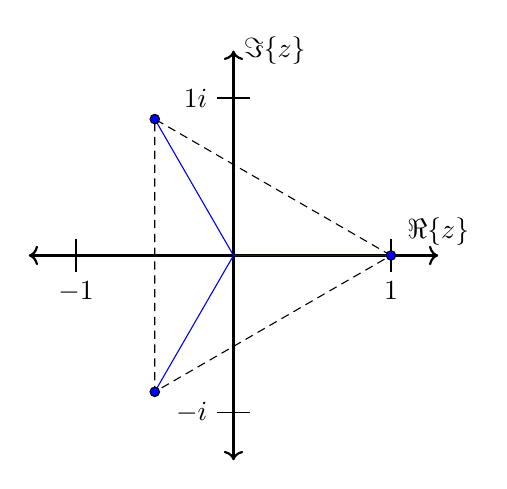
\begin{tikzpicture}[scale=2]
        % Coordinates for the three roots and origin.
        \coordinate (O)  at (0.0, 0.0);
        \coordinate (Z1) at (1.0, 0.0);
        \coordinate (Z2) at (-0.5, 0.866);
        \coordinate (Z3) at (-0.5, -0.866);

        % Axes:
        \begin{scope}[thick]
            \draw[<->] (-1.3, 0) to (1.3, 0) node[above] {$\Re\{z\}$};
            \draw[<->] (0, -1.3) to (0, 1.3) node[right] {$\Im\{z\}$};
        \end{scope}

        % Axes labels:
        \draw (1, 3pt)  to (1, -3pt)  node [below] {$1$};
        \draw (-1, 3pt) to (-1, -3pt) node [below] {$-1$};
        \draw (3pt, 1)  to (-3pt, 1)  node [left]  {$1{i}$};
        \draw (3pt, -1) to (-3pt, -1) node [left]  {$-i$};

        % Draw the cubed roots of unity.
        \draw[blue] (O) to (Z1);
        \draw[blue] (O) to (Z2);
        \draw[blue] (O) to (Z3);

        % Connect the three roots with dashed lines.
        \draw[densely dashed, thin] (Z1) to (Z2) to (Z3) to cycle;

        % Draw dots to mark the points.
        \draw[fill=blue] (Z1) circle (0.3mm);
        \draw[fill=blue] (Z2) circle (0.3mm);
        \draw[fill=blue] (Z3) circle (0.3mm);
    \end{tikzpicture}
    \caption{The Third Roots of Unity}
    \label{fig:ThirdRootsOfUnity}
\end{figure}

\begin{problem}
    Let $V$ be the vector space with basis:
    \begin{equation}
        \{ v_s \vert \text{ s is a $2$-element subset of }\{1,2,3,4\}\}
    \end{equation}
    \begin{enumerate}
        \item[(a)]
            $S_4$ acts on $V$ by $v_s\cdot\sigma = v_{s\cdot\sigma}$. Determine the character
            $\chi$ of this representation and write $\chi$ as a sum of irreducible representations.
            \begin{solution}
        
                First, notice that $V$ has 6 basis elements:
                \begin{equation}
                    \big\{\,
                        \{1,\,2\},\,
                        \{1,\,3\},\,
                        \{1,\,4\},\,
                        \{2,\,3\},\,
                        \{2,\,4\},\,
                        \{3,\,4\}\,
                    \big\}
                \end{equation}
                $S_4$ has five conjugacy class: $1^4, 2 1^2, 2^2, 31, 4$. 
                First, do $1^4$. $\phi(1^4)$ is the 6x6 identity matrix, because it sends each basis
                element to itself. Thus, the trace is 6. 
                For the remaining conjugacy classes, choose a representative element and count how many
                basis elements it fixes. In $2^2$, $(1,2)(3,4)$ fixes $\{1,2\}$ and $\{3,4\}$, so
                $\chi(2^2) = 2$.  The final character for conjugacy classes $1^4, 2 1^2, 2^2, 31, 4$ is
                6 2 2 0 0. This character can be expressed as :
                \begin{table}[H]
                    \centering
                    \begin{tabular}{rrrrrr}
                          & 6 & 2 & 2 & 0 & 0\\ 
                        \hline 
                          & 1 & 1 & 1 & 1 & 1\\
                        + & 3 & 1 & -1 & 0 & -1 \\
                        + & 2 & 0 & 2 & -1 & 0
                    \end{tabular}
                \end{table}
            \end{solution}
        \item[(b)]
            Repeat the above for $V$ having a basis indexed by $3$-element subsets
            of $\{1,2,3,4\}$.
            \begin{solution}
                Now there are four basis elements:
                \begin{equation}
                    \big\{\,
                        \{1,\,2,\,3\},\,
                        \{1,\,2,\,4\},\,
                        \{1,\,3,\,4\},\,
                        \{2,\,3,\,4\}\,
                    \big\}
                \end{equation}
                Once again, we need to count the number of basis elements fixed by each conjugacy class to
                get the character. This time, the final character for conjugacy classes $1^4, 2 1^2, 2^2, 31,
                4$ is 4 2 0 1 0.
                \begin{table}[h]
                \centering
                    \begin{tabular}{rrrrrr}
                           & 4 & 2 & 0 & 1 & 0  \\ 
                           \hline 
                           & 1 & 1 & 1 & 1 & 1 \\
                         + & 3 & 1 & -1 & 0 & -1
                    \end{tabular}
                \end{table}
            \end{solution}
    \end{enumerate}
\end{problem}
\begin{problem}
    Recall the M\"{o}bius function $\mu$ of a poset $\mathcal{P}$ that was explored by Team Stanley:
    \begin{equation}
        \mu(x,y)=
        \begin{cases}
            1&x=y\\
            -\sum_{x\leq z < y}\mu(x,z)&\text{else}
        \end{cases}
    \end{equation}
    Let $\mathcal{D}$ denote the poset of all divisors of $n$ ordered by division ($u\leq v$ if $u|v$).
    \begin{enumerate}
        \item[(a)]
            Draw the poset of divisors of $12$, $\mathcal{D}_{12}$,
            and next to each vertex $u$ write $\mu(1,u)$.
            \begin{solution}
                Note: $\mu(1,u)$ is given in parenthesis next to $u$.
                \begin{figure}[H]
                    \centering
                    \begin{tikzcd}
                        &&12(0)\arrow[ld,dash]\arrow[rd,dash]&\\
                        &6(+1)\arrow[ld,dash]\arrow[rd,dash]&&4(0)\arrow[ld,dash]\\
                        3(-1)\arrow[rd,dash]&&2(-1)\arrow[ld,dash]&\\
                        &1(+1)&&
                    \end{tikzcd}
                    \caption{Solution for Problem 3}
                    \label{fig:SolutionProblem3}
                \end{figure}
            \end{solution}
        \item[(b)]
            In $\mathcal{D}_{n}$, show that $\mu(x,y)=M(\frac{y}{x})$, where $M(u)$ is the
            number theoretic M\"{o}bius function:
            \begin{equation}
                M(u)=
                \begin{cases}
                    1&u=1\\
                    (-1)^r&\text{if $u$ is a product of $r$ distinct primes}\\
                    0&\text{otherwise}
                \end{cases}
            \end{equation}
            \begin{solution}
                If $x=y$, then $y/x=1$ to $\mu(x,y)$ and $M(y/x)$ agree here.
                Otherwise, writing $x=p_{1}^{r_{1}}\cdots{p}_{m}^{r_{m}}$ and
                $y=x\cdot{q}^{s_{1}}\cdots{q}^{s_{m}}$ (since $x$ and $y$ are
                comparable and hence $x|y$), we get $y/x=q^{s_{1}}\cdots{q}^{s_{m}}$
                so $M(y/x)=(-1)^{N}$ where $N$ is the sum of the $r_{k}$
                assuming all of them are zero or one, and $M(y/x)=0$ otherwise. But
                this also gives us all of the elements between $x$ and $y$,
                namely $x$, $xq_{1}$, and so on. If the primes are distinct, we
                get $(-1)^{N}$ where $N$ is again the number of distinct primes. If
                there is multiplicity in one of the primes, then there are two ways
                to get from $x$ to $y$ in the lattice, and these paths will cancel
                in the sum, resulting in zero.
            \end{solution}
        \item[(c)]
            Show that $M(u)$ is the sum of the primitive $u^{th}$ roots of unity.
            \begin{solution}
                From the definition of $M$, we have that:
                \begin{equation}
                    \sum_{k|u}M(n)=
                    \begin{cases}
                        1,&u=1\\
                        0,&\textrm{else}
                    \end{cases}
                \end{equation}
                Hence:
                \begin{subequations}
                    \begin{align}
                        \sum_{\textrm{GCD}(n,u)=1}\exp(2\pi{i}n/u)
                        &=\sum_{n=1}^{u}\sum_{k|\textrm{GCD(n,u)}}M(k)\exp(2\pi{i}n/u)\\
                        &=\sum_{k|\textrm{GCD(n,u)}}M(k)\sum_{n=1}^{u}\exp(2\pi{i}n/u)\\
                        &=\sum_{k|u}M(k)\sum_{m=1}^{u/k}\exp(2\pi{i}nm/u)\\
                    \end{align}
                \end{subequations}
                And this last sum is only non-zero when $k=u$, so we get:
                \begin{equation}
                    M(u)=\sum_{\text{GCD}(n,u)=1}\exp(2\pi{i}n/u)
                \end{equation}
            \end{solution}
    \end{enumerate}
\end{problem}

\begin{problem} Let $E$ be the graph obtained from $G$ by deleting every edge other than $e$, but keeping all the vertices. Let $D_r$ be the subspace generated by basis vectors indexed by the ordered set partitions $(B_1,\dots,B_{r+2})$ such that no $B_i$ contains the edge $e$.

(Recall that $\Delta_r(G)$ is defined to be the vector space spanned by all ordered set partitions $(B_1, \dots, B_{r+1})$ of the vertex set of $G$ such that \emph{at least one} $B_i$ contains an edge of $G$. )

\begin{enumerate}
    \item[(a)] Show that $\Delta_r(G) = D_r \oplus \Delta_r(E)$.
    \begin{solution}
This is immediate as the basis of $\Delta_r(G)$ splits as those basis elements which are indexed by some partition not containing $e$ and those indexed by a partition containing only $e$. Explicitly, corresponds to taking the term-wise union of the two ordered set partitions on the RHS.
\end{solution}
    \item[(b)] Show that $\Delta_r(G-e)\cong D_r \oplus \left(\Delta_r(G-e)\cap \Delta_r(E) \right)$
    \begin{solution}
This follows from the observation that an ordered set partition of vertices of $G-e$ could still contain the edge $e$, and this occurs only when it was obtained from an ordered set partition of vertices of $G$ that have only the edge $e$. Again, this corresponds to taking the term-wise union of the ordered set partitions on the RHS.
\end{solution}
    \item[(c)] Show that $\Delta_r(G-e)\cap \Delta_r(E) \cong \Delta_r(G/e)$
    \begin{solution}
        This follows from the observation that an ordered set
        partition of vertices of $G/e$ that contains an edge must
        contain an edge in addition to the ``edge'' $e$, thus is a set
        partition of vertices of $G-e$ containing an edge and of
        vertices of $E$ that contain the only edge $e$.

Any $(B_1, \dots, B_{r+2})$ on LHS must have some $B_i$ containing the edge $e$ (and must also contain some other edge from $G$ in some $B_j)$. Thus $B_i$ contains at least two vertices, the endpoints $u,v$ of $e$. So when we compress $e$ to get $G/e$, we can get a corresponding $B_i'$ containing vertex $uv$, and can carry along $B_j$ (containing edge $\neq e$) as-is, unencumbered by contracting $e$. The key part is that $B_i'$ is not empty, so we still have the correct number of sets in our partition on the RHS, and that $B_j$ DOES contain an edge of $G/e$.

\end{solution}
    \item[(d)] Conclude that $\Delta_r(G) \oplus \Delta_r(G/e)\cong \Delta_r(G-e)\oplus\Delta_r(E)$
    \begin{solution}
This follows from the computation $$\Delta_r(G)\oplus\Delta_r(G/e) \cong D_r \oplus \Delta_r(E) \oplus\left(\Delta_r(G-e)\cap \Delta_r(E) \right) \text{ by (a) and (c)}$$ $$ \cong \Delta_r(E) \oplus D_r \oplus\left(\Delta_r(G-e)\cap \Delta_r(E) \right) \cong \Delta_r(E) \oplus \Delta_r(G-e) \text{ by (b)}$$
\end{solution}
\item[(e)] Let $S_{r+2}$ act on the sequences $(B_1,B_2,\dots,B_{r+2})$ by $$(B_1,B_2,\dots,B_{r+2}))\cdot\sigma = (B_{1\cdot\sigma},B_{2\cdot\sigma},\dots,B_{(r+2)\cdot\sigma})).$$ Confirm that the isomorphism in part (d) above is an isomorphism of $S_{r+2}$-modules.
\begin{solution}
All the isomorphisms in (d) are $S_{r+2}$-module isomorphisms, as taking the union and then acting by a permutation or permuting and then taking a term-wise union are the same. Hence the isomorphism in part (d) above is an $S_{r+2}$-module isomorphism.
\end{solution}
\end{enumerate}
\end{problem}



\begin{problem}
Show that the symmetric group $S_m$ is generated by the adjacent transpositions $$S_m = \langle (1,2), (2,3),\dots,(m-1,m)\rangle$$
\end{problem}
\begin{solution}
We note that $S_m$ is generated by transpositions. Thus it suffices to show that we can produce any transposition $(i,j)$ with $i<j$ as a product of adjacent transpositions. We also note that conjugating a permutation $(\dots,j,\dots)$ by $(i,j)$ relabels the entry $j$ with $i$. But then the problem reduces to the equality $$(i,j) = (j-1,j)\cdots(i+1,i+2)\cdot(i,i+1)\cdot(i+1,i+2)\cdots(j-2,j-1)\cdot(j-1,j)$$


Recall: Arbitrary cycle in $S_m$ can be realized as the product of transpositions: 
\[(a_1, a_2, \dots, a_k) = (a_1, a_2)(a_2, a_3) \dots (a_{k-1}, a_k)\]
(read right-to-left). Since every element of $S_m$ can be written as product of disjoint cycles, we are done.

\end{solution}
\end{document}